\chapter{Main Body}
\label{cha:Main Body}


\section{''Pflichtenheft''}
\label{sec:Pflichtenheft}

\subsubsection{Cost}
I've already bought two \acs{devboard}s one of them stays at \acs{tbz} and the other is at home. One of these boards was paid by Mr. Malacarne. Further expenses from the \acs{pcb} will be paid by me and shouldn't exceed about 50 CHF, as the \acs{hw} isn't that complicated.

\subsubsection{Time}
The most time of the project I will work at home because it's a rather big project to execute in one semester. I will also have much time in the fall holidays to work on it. The project will approximately take 100h to complete. Also the more detailed timeplan is in chapter: [\ref{sec:GANTT Chart}]

\subsubsection{Tools}
To realize this project I will mainly use, the \acs{sw} STM32CubeIDE with \acs{hal} and Altium Designer. The documentation is written in LaTeX in VSCode. And I'm planning to order the \acs{pcb} on JLCPCB and I will populate and reflow the PCB at ETHZ, where I'm also allowed to use the measurement equipment for the HW tests.


\subsubsection{Technical Details}
\begin{table}[H]
    \centering
    \label{tab:Technical Details}
\begin{tabular}{||c || c | c | c | c  || c ||} 
 \hline
 value &  min. & typ. & max. & unit & description \\ [0.5ex] 
 \hline\hline
  supply voltage & & 5 & & V & \\ 
 \hline
\end{tabular}
    \caption{Technical Details}
\end{table}

\newpage


\section{Extension PCB}
\label{sec:Extension PCB}



\subsection{STMod+}
Interface from DevBoard to Extension PCB. 

\begin{itemize}
    \item 5V Supply
    \item SPI 
    \item I\textsubscript{2}C
    \item ADC
    \item Interrupt
    \item PWM
    \item GPIOs
\end{itemize}

\begin{figure}[H]
	\centering
	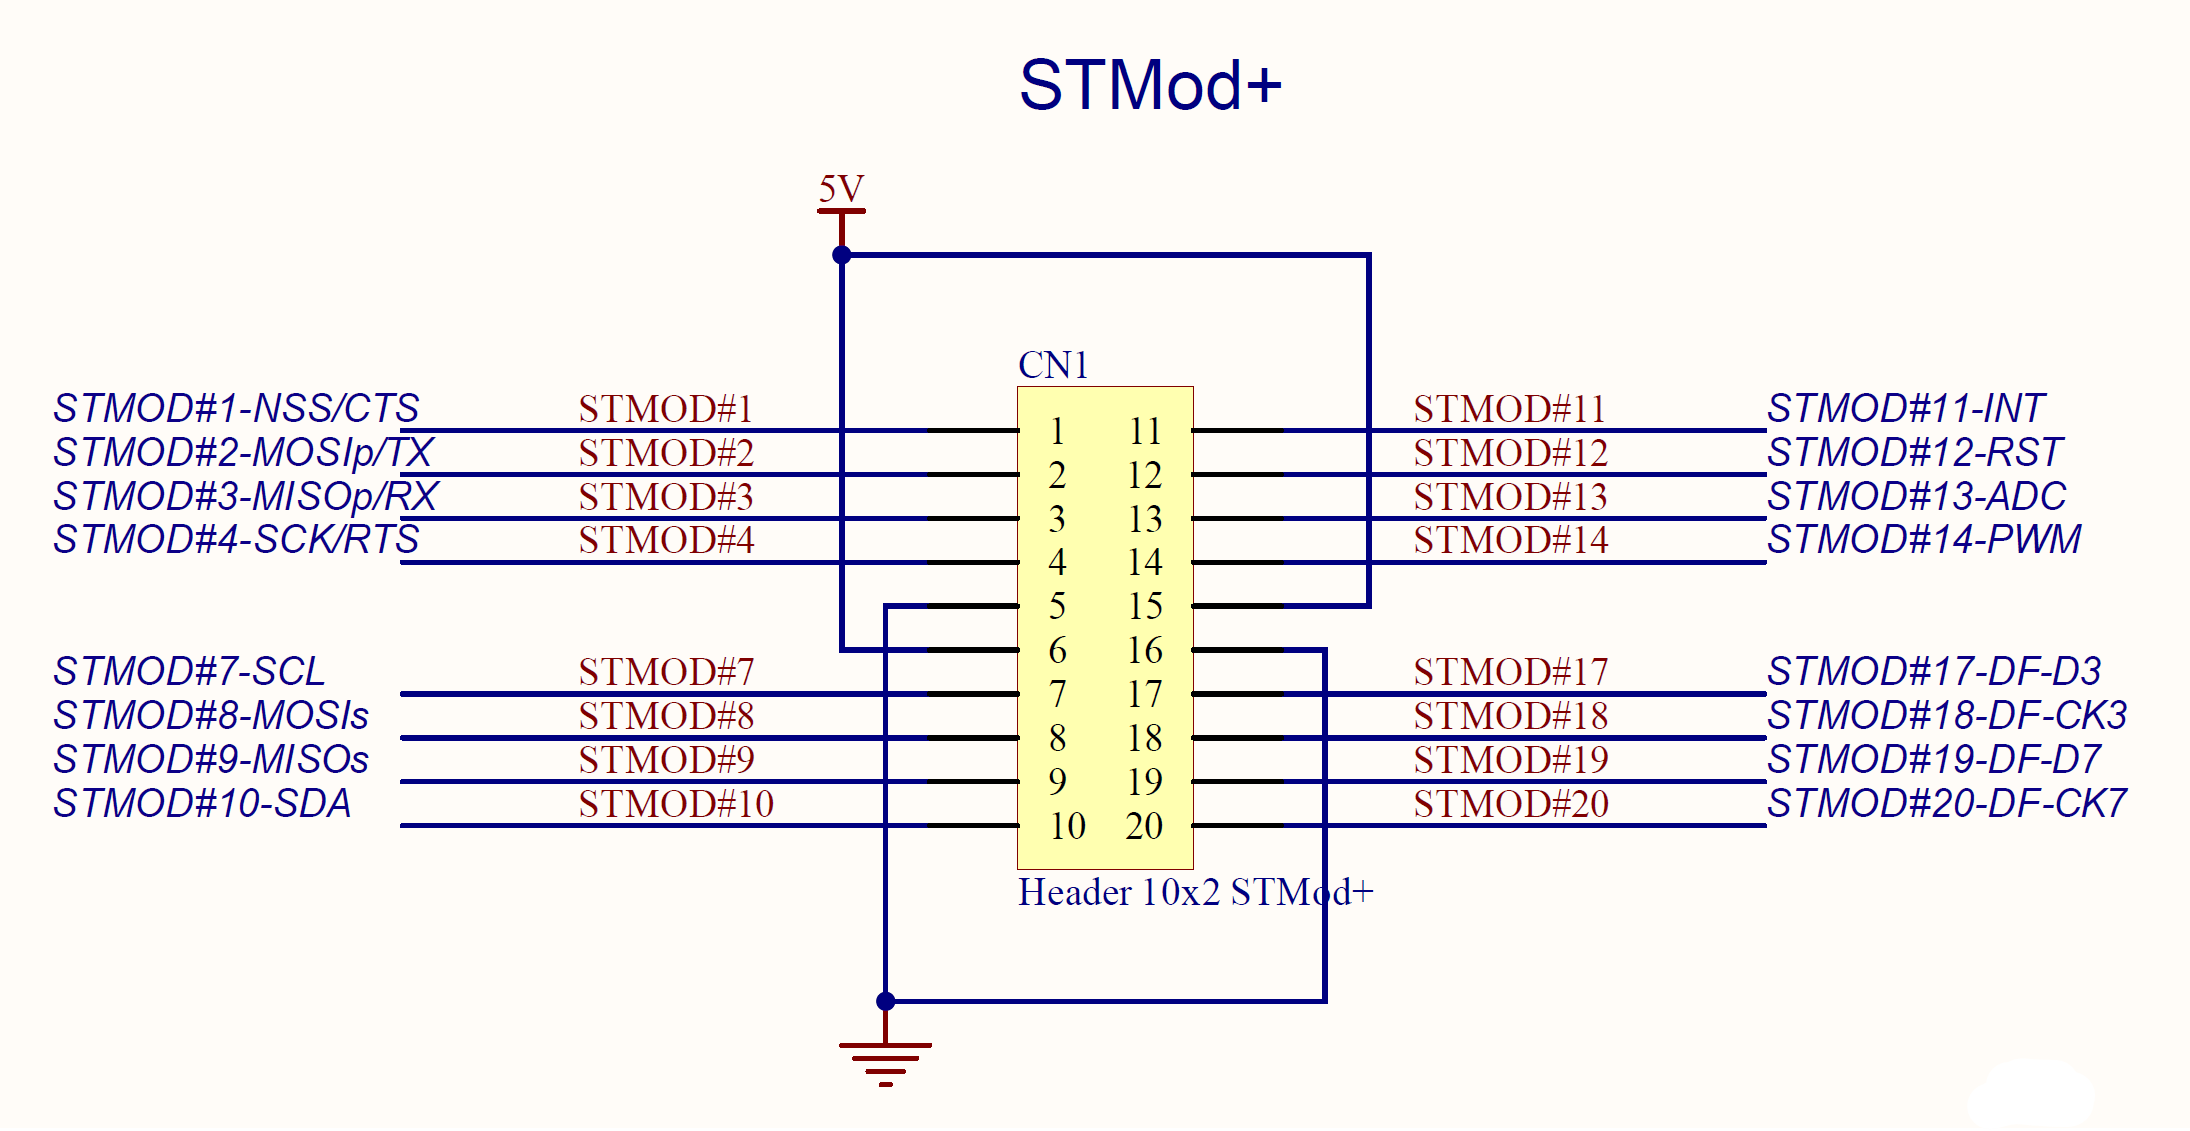
\includegraphics[width=13cm]{Resources/Pictures/STMOD_Interface.png}
	\caption{STMod+ Interface}
	\label{fig:STMod+ Interface}
\end{figure}






\subsection{Block Diagram}




\begin{figure}[H]
	\centering



    \tikzstyle{block} = [draw, fill=white, rectangle, 
    minimum height=3em, minimum width=6em]
    \tikzstyle{sum} = [draw, fill=white, circle, node distance=1cm]
    \tikzstyle{input} = [coordinate]
    \tikzstyle{output} = [coordinate]
    \tikzstyle{pinstyle} = [pin edge={to-,thin,black}]

\begin{tikzpicture}[auto, node distance=2cm,>=latex']

    \node [input, name=input] {};
    \node [sum, right of=input] (sum) {};
    \node [block, right of=sum] (controller) {Controller};
    \node [block, right of=controller, pin={[pinstyle]above:D},
            node distance=3cm] (system) {System};

    \draw [->] (controller) -- node[name=u] {$u$} (system);
    \node [output, right of=system] (output) {};
    \node [block, below of=u] (measurements) {Measurements};

    \draw [draw,->] (input) -- node {$r$} (sum);
    \draw [->] (sum) -- node {$e$} (controller);
    \draw [->] (system) -- node [name=y] {$y$}(output);
    \draw [->] (y) |- (measurements);
    \draw [->] (measurements) -| node[pos=0.99] {$-$} 
        node [near end] {$y_m$} (sum);
\end{tikzpicture}

    \vspace{1cm}

	\caption{Extension PCB Block Diagram}
	\label{fig:Extension PCB Block Diagram}
\end{figure}